\documentclass{article}
\usepackage{graphicx}
\usepackage{authblk}
\usepackage{amsmath}
\usepackage{textcomp}

\begin{document}
\title{THEORETICAL NEUROSCIENCE \\ EXERCISE 6}
\date{\today}
\author[1]{\c{S}eyma Bayrak\thanks{seyma.bayrak@st.ovgu.de}}
\affil[1]{\footnotesize  Otto von Guericke University of Magdeburg}
\maketitle

\section{Introduction}

In visual cortex, neurons response each time differently, when they are triggered by identical stimuli. Instead of characterizing neruon`s response by triggering it only once, the neuron is driven several times by the same stimulus. At the end, an average response is found out by simple statistical methods.\\

The response of neuron does not only depend on stimuli, but also which parts of visual system are triggered. For example, any input driven out of \textbf{receptive fields} cannot be transferred into a real signal. The receptor fields have also subgroups among themselves; \textbf{ON/OFF regions}. Whereas ON centers respond to onset of light, OFF centers respond to onset of dark. ON and OFF regions are not arbitrarily localized by surrounding each other.\\ 

The final term to be defined is \textbf{tuning curve}; the average response of a neuron as a function of one particular stimulus parameter. In this exercise, the two "mysterious neurons" are driven by different types of stimulus. The purpose of this assignment is to repeat each stimuli many times for each of two neurons and to get their corresponding tuning curves.

\section{Programming Assignment}

We have provided five functions creating five different stimuli types. \textbf{OnSpot} and \textbf{OffSpot} functions' inputs are only the user defined array size \textbf{n}, these functions represent trigger of neuron at ON and OFF regions. \textbf{OnBar} and \textbf{OffBar} functions get the parameters \textbf{n} and \textbf{theta}, "theta" represents the positon of stimuli to the visual cortex here. Finally, the function \textbf{WhiteNoise} depends also only on array size \textbf{n}, it is a stimulus identical to the noise in the environment. The programming assignment is explained step by step below for two imaginary neurons \textbf{MysteriousNeuron1} and \textbf{MysteriousNeuron2}. \\ 

\setcounter{tocdepth}{1}
\textbf{1.} \textbf{Stimulating repeatedly with bright bars:} The stimuli is called as $S=OnBar(n, theta)$. The array size is chosen as n=50 and angle theta, $\theta$, is between 0 and $\pi$. The scalar output to this stimuli is called as $r=MysteriousNeuron1(S)$ for the first neuron and $r=MysteriousNeuron2(S)$ for the second neuron. \\

\textbf{r} is a scalar value, not an array! By stimulation neuron many times, all the "r" values recorded inside a \textit{for loop}. Then the following formulas are used to get an average response, "tuning curve" so to say. 

\begin{equation}
 \langle r(\theta) \rangle=\frac{1}{N} \sum\limits_{i=1}^{N}r_i(\theta) \,\,\,\,\,\,{average\,\,\,of\,\,\,stimulus\,\,\,at\,\,\,various \,\,\,angles}
\end{equation}

\begin{equation}
 \sigma_r(\theta)=\sqrt{ \frac{N (\langle r^2 \rangle-\langle r \rangle ^2 ) }{N-1}  }\,\,\,\,\,\,{standart\,\,\,deviation\,\,\,of\,\,\,average\,\,\,response}
\end{equation}

In MATLAB assignment, \textit{N} value, how many times the neuron is stimulated is typed as 300. The following graphs for both neurons are eliminated.

\begin{center}
 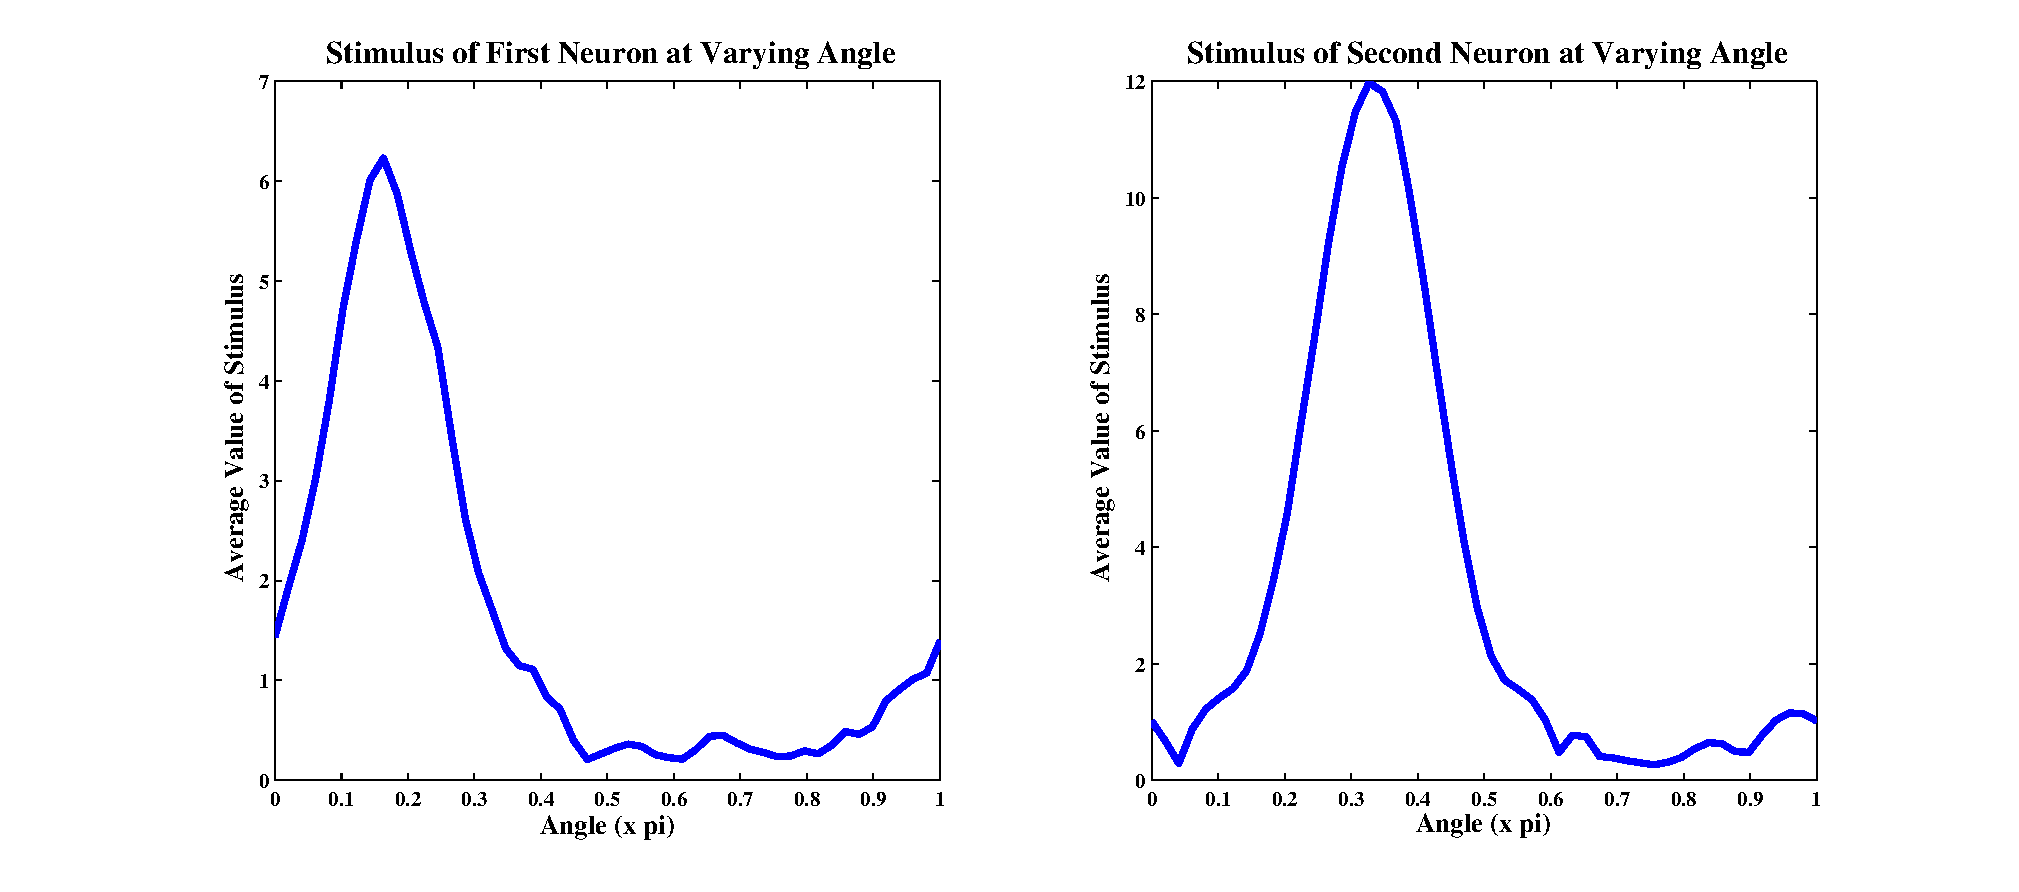
\includegraphics[width=\textwidth]{f1_on.eps}
 % q7.eps: 0x0 pixel, 300dpi, 0.00x0.00 cm, bb=  -86   231   682   610
\begin{footnotesize}Graph 1, The average of responses of two mysterious neurons driven by bright bars. The angle $\theta$ is placed on all graphs as at x axis, as multiples of $\pi$.\end{footnotesize}
\end{center}

\begin{center}
 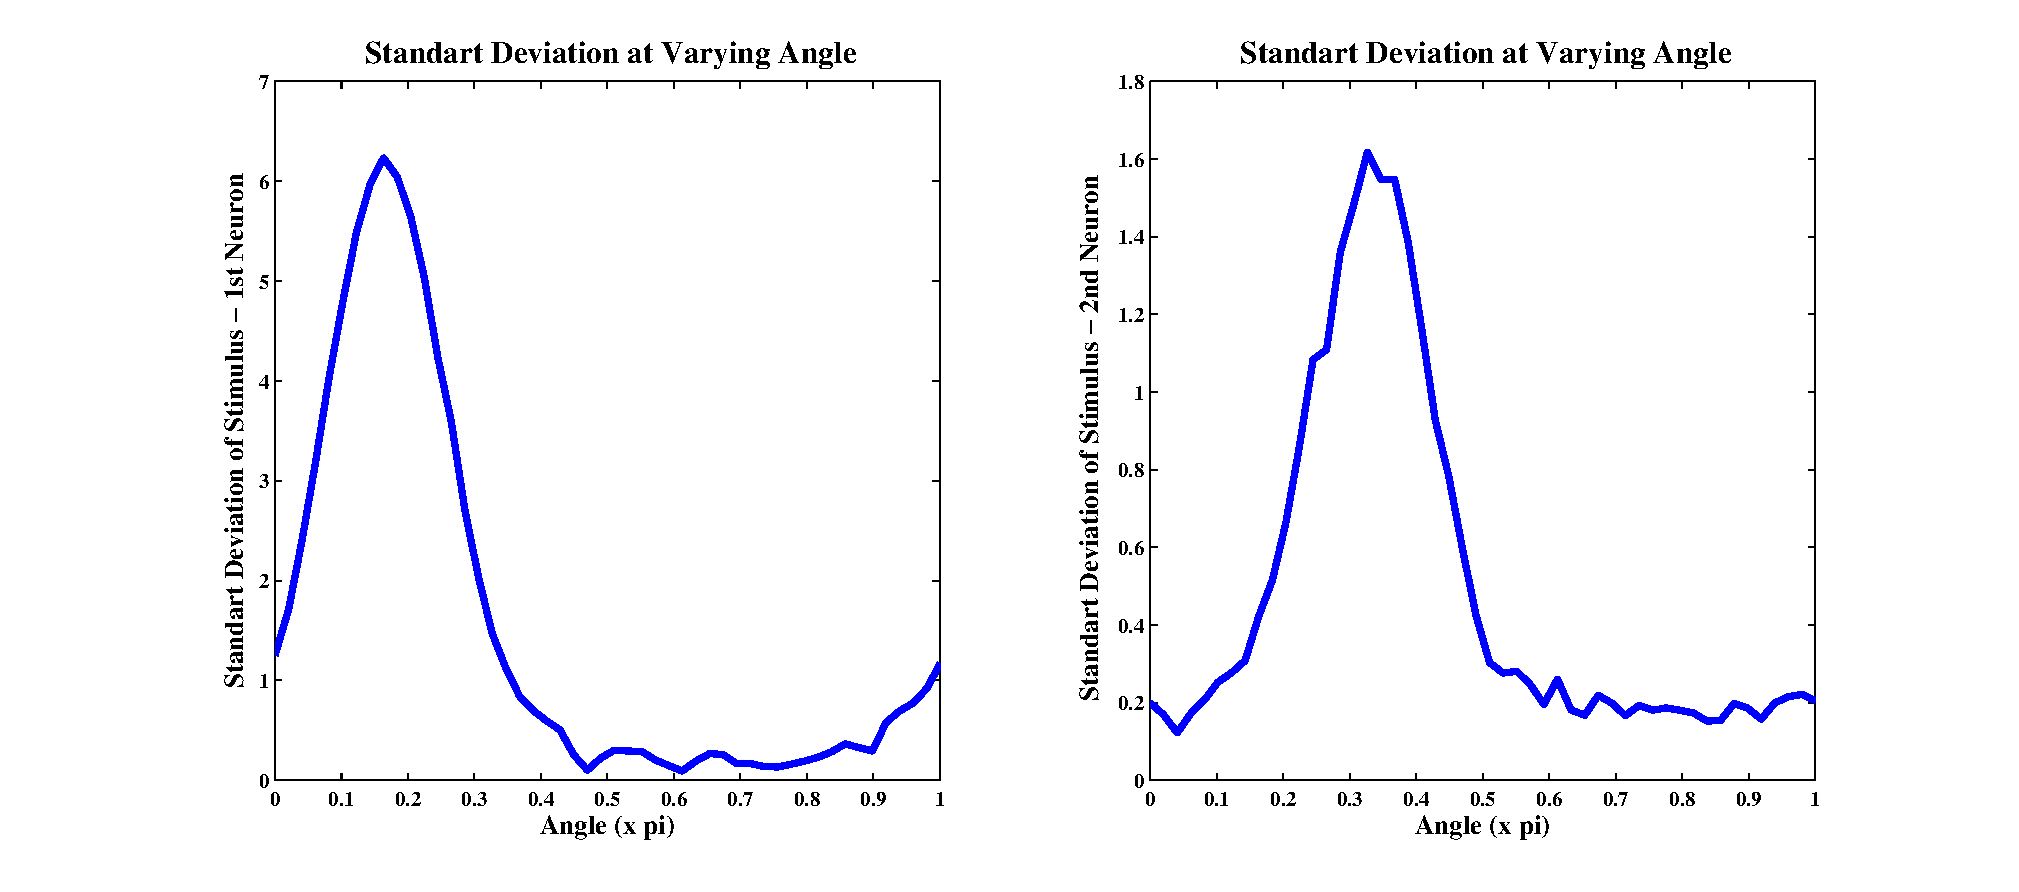
\includegraphics[width=\textwidth]{std_on.eps}
 % q7.eps: 0x0 pixel, 300dpi, 0.00x0.00 cm, bb=  -86   231   682   610
\begin{footnotesize}Graph 2, The standart deviations of average of responses of two mysterious neurons driven by bright bars. \end{footnotesize}
\end{center}

\setcounter{tocdepth}{1}
\textbf{2.Stimulating repeatedly with dark bars:} The same procedure in step 1 is repeated. This time the called stimulus function is $S=OffBar(n, theta)$. The following graphs are eliminated.

\begin{center}
 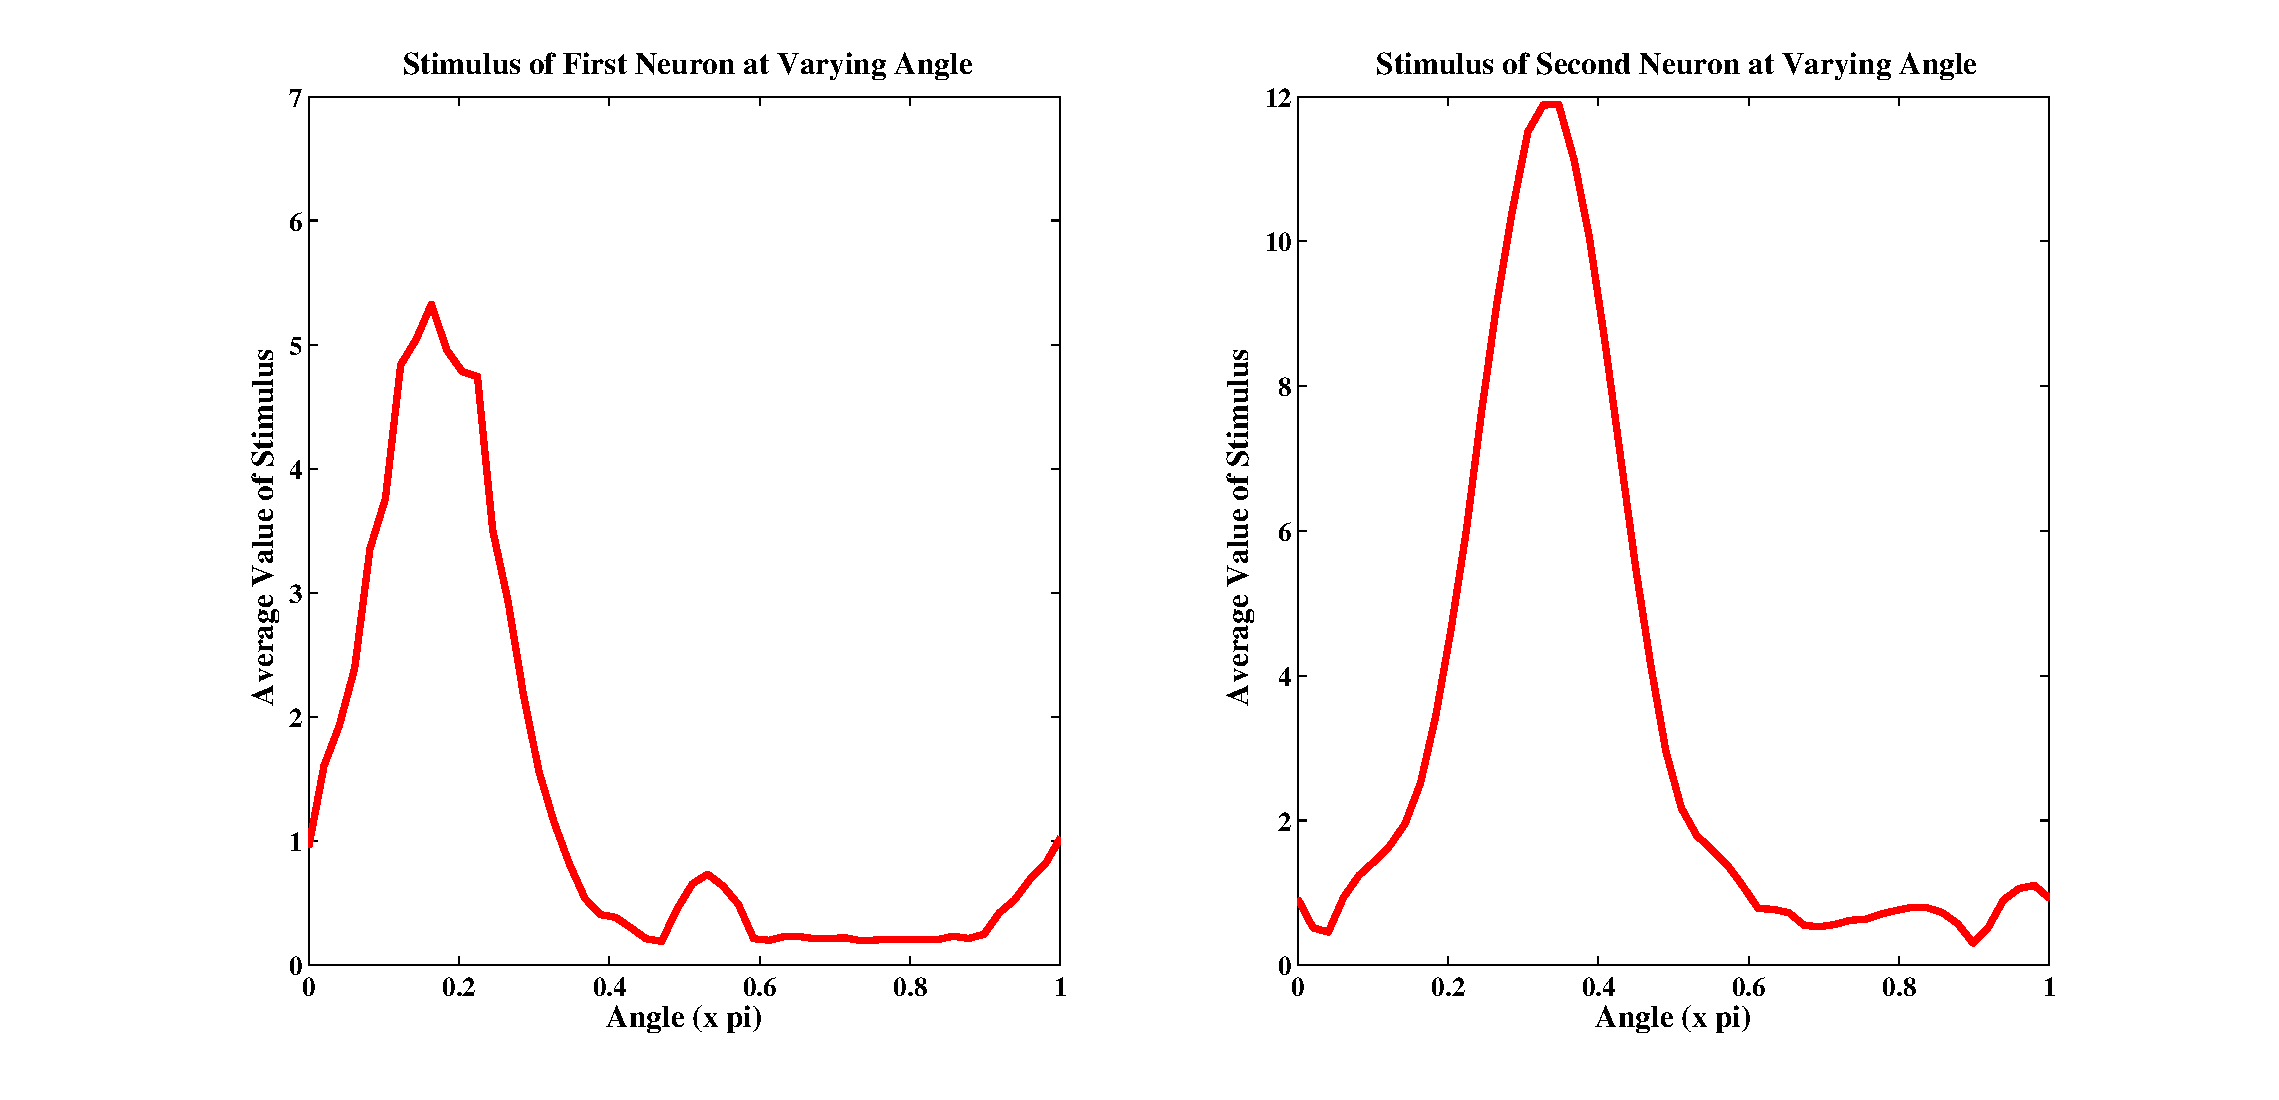
\includegraphics[width=\textwidth]{f1_off.eps}
 % q7.eps: 0x0 pixel, 300dpi, 0.00x0.00 cm, bb=  -86   231   682   610
\begin{footnotesize}Graph 3, The average of responses of two mysterious neurons driven bar dark bars. \end{footnotesize}
\end{center}

\begin{center}
 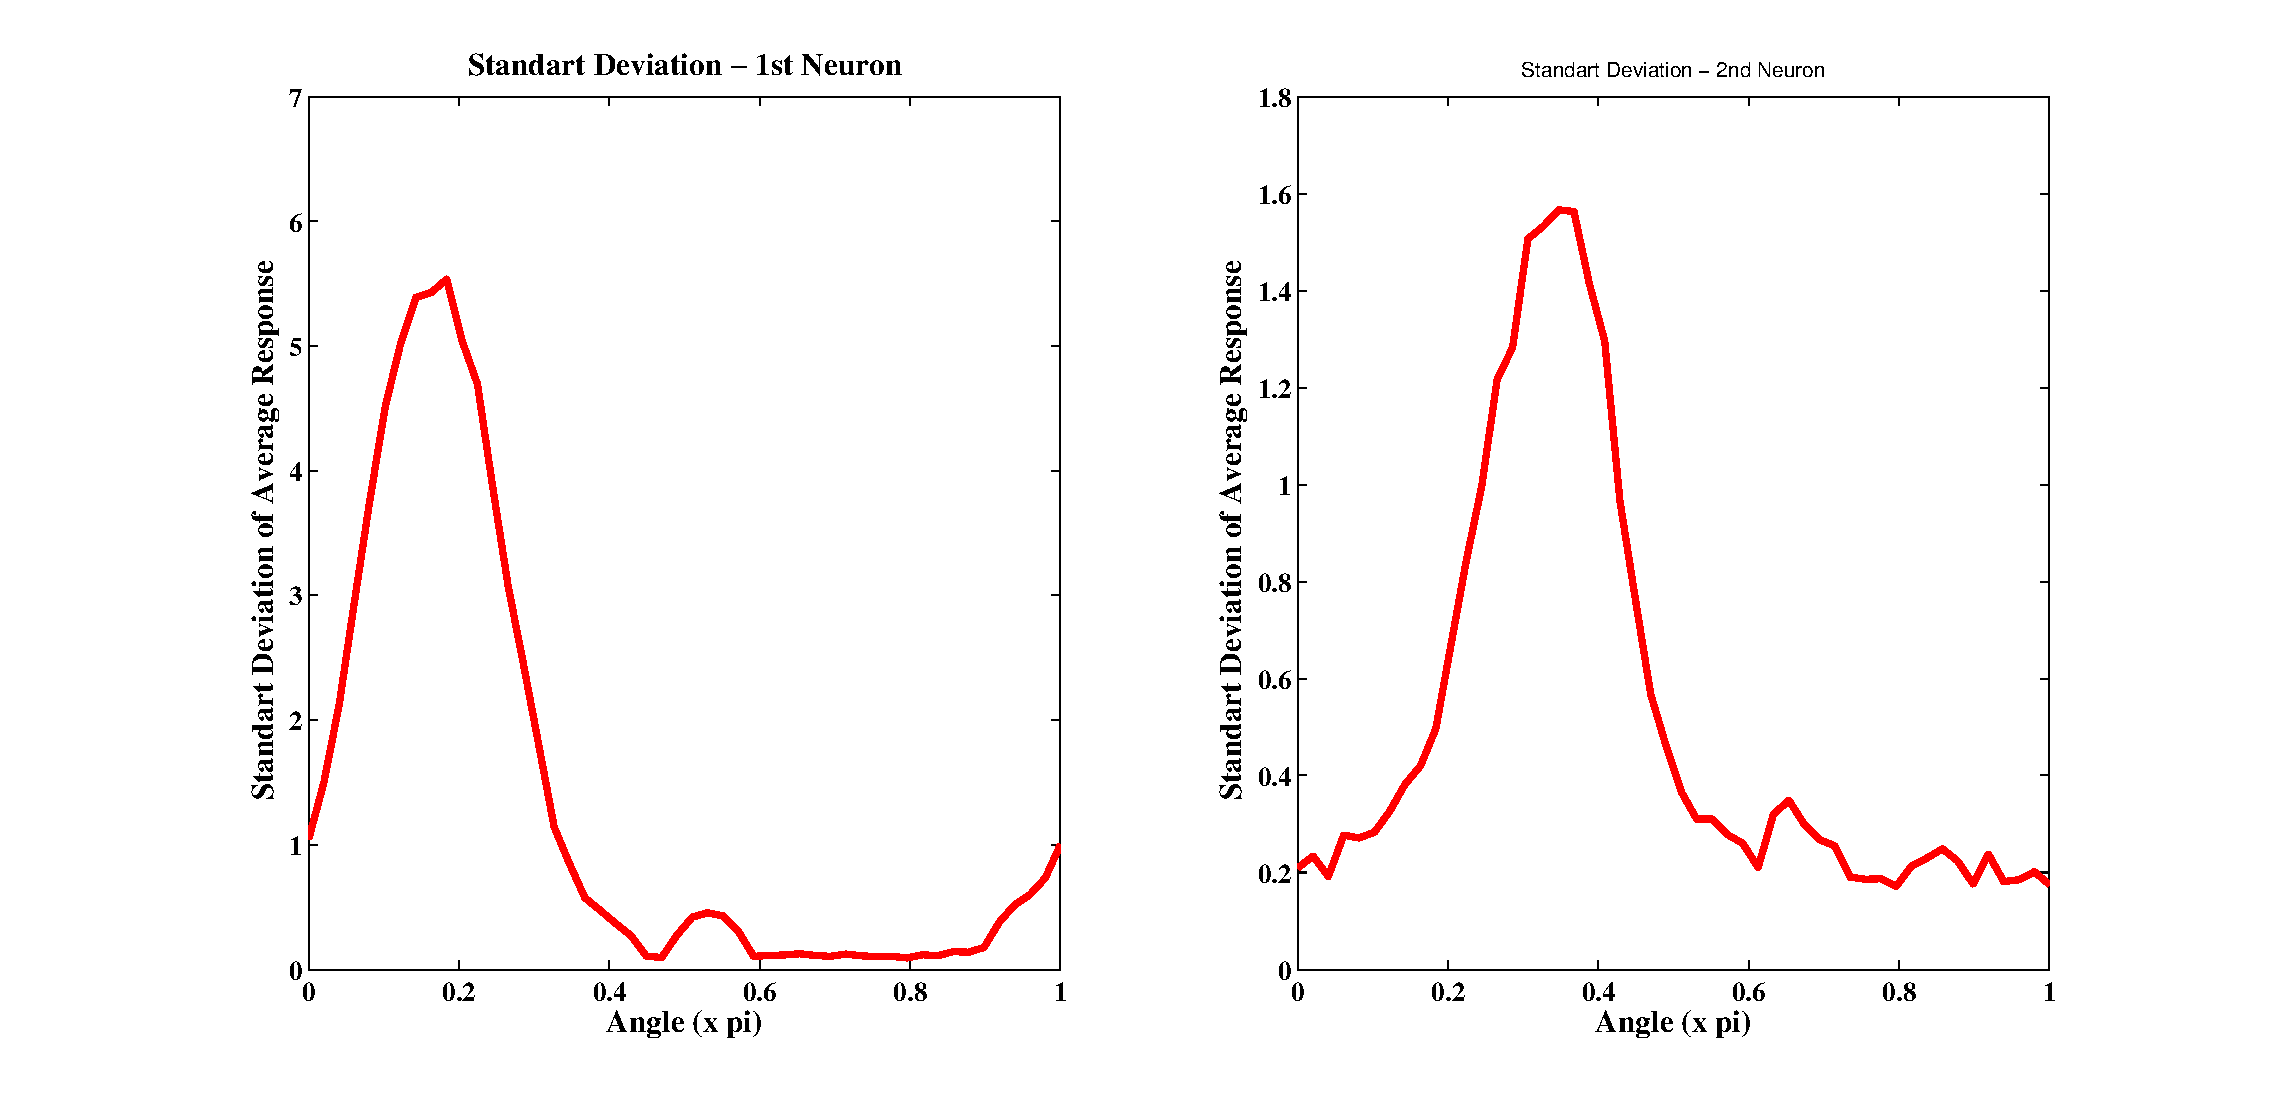
\includegraphics[width=\textwidth]{std_off.eps}
 % q7.eps: 0x0 pixel, 300dpi, 0.00x0.00 cm, bb=  -86   231   682   610
\begin{footnotesize}Graph 4, The standart deviations of average of responses of two mysterious neurons driven by dark bars. \end{footnotesize}
\end{center}

\setcounter{tocdepth}{1}
\textbf{3.Stimulating repeatedly with bright spots:} The stimuli function is $S=OnSpot(n)$. The scalar response r is called for two neurons again. This time a response weighted average of the presented stimuli computed as in the following equation. The graphs can be shown below, they are drawn by the command \textbf{pcolor} on MATLAB. 

\begin{equation}
 S'=\frac{\sum\limits_{i}^{N}S_ir_i}{\sum\limits_{i}^{N}r_i}\,\,\,\,\,\,{weigted\,\,\,average\,\,\,of\,\,\,at\,\,\,presented \,\,\,stimuli}
\end{equation}

\begin{center}
 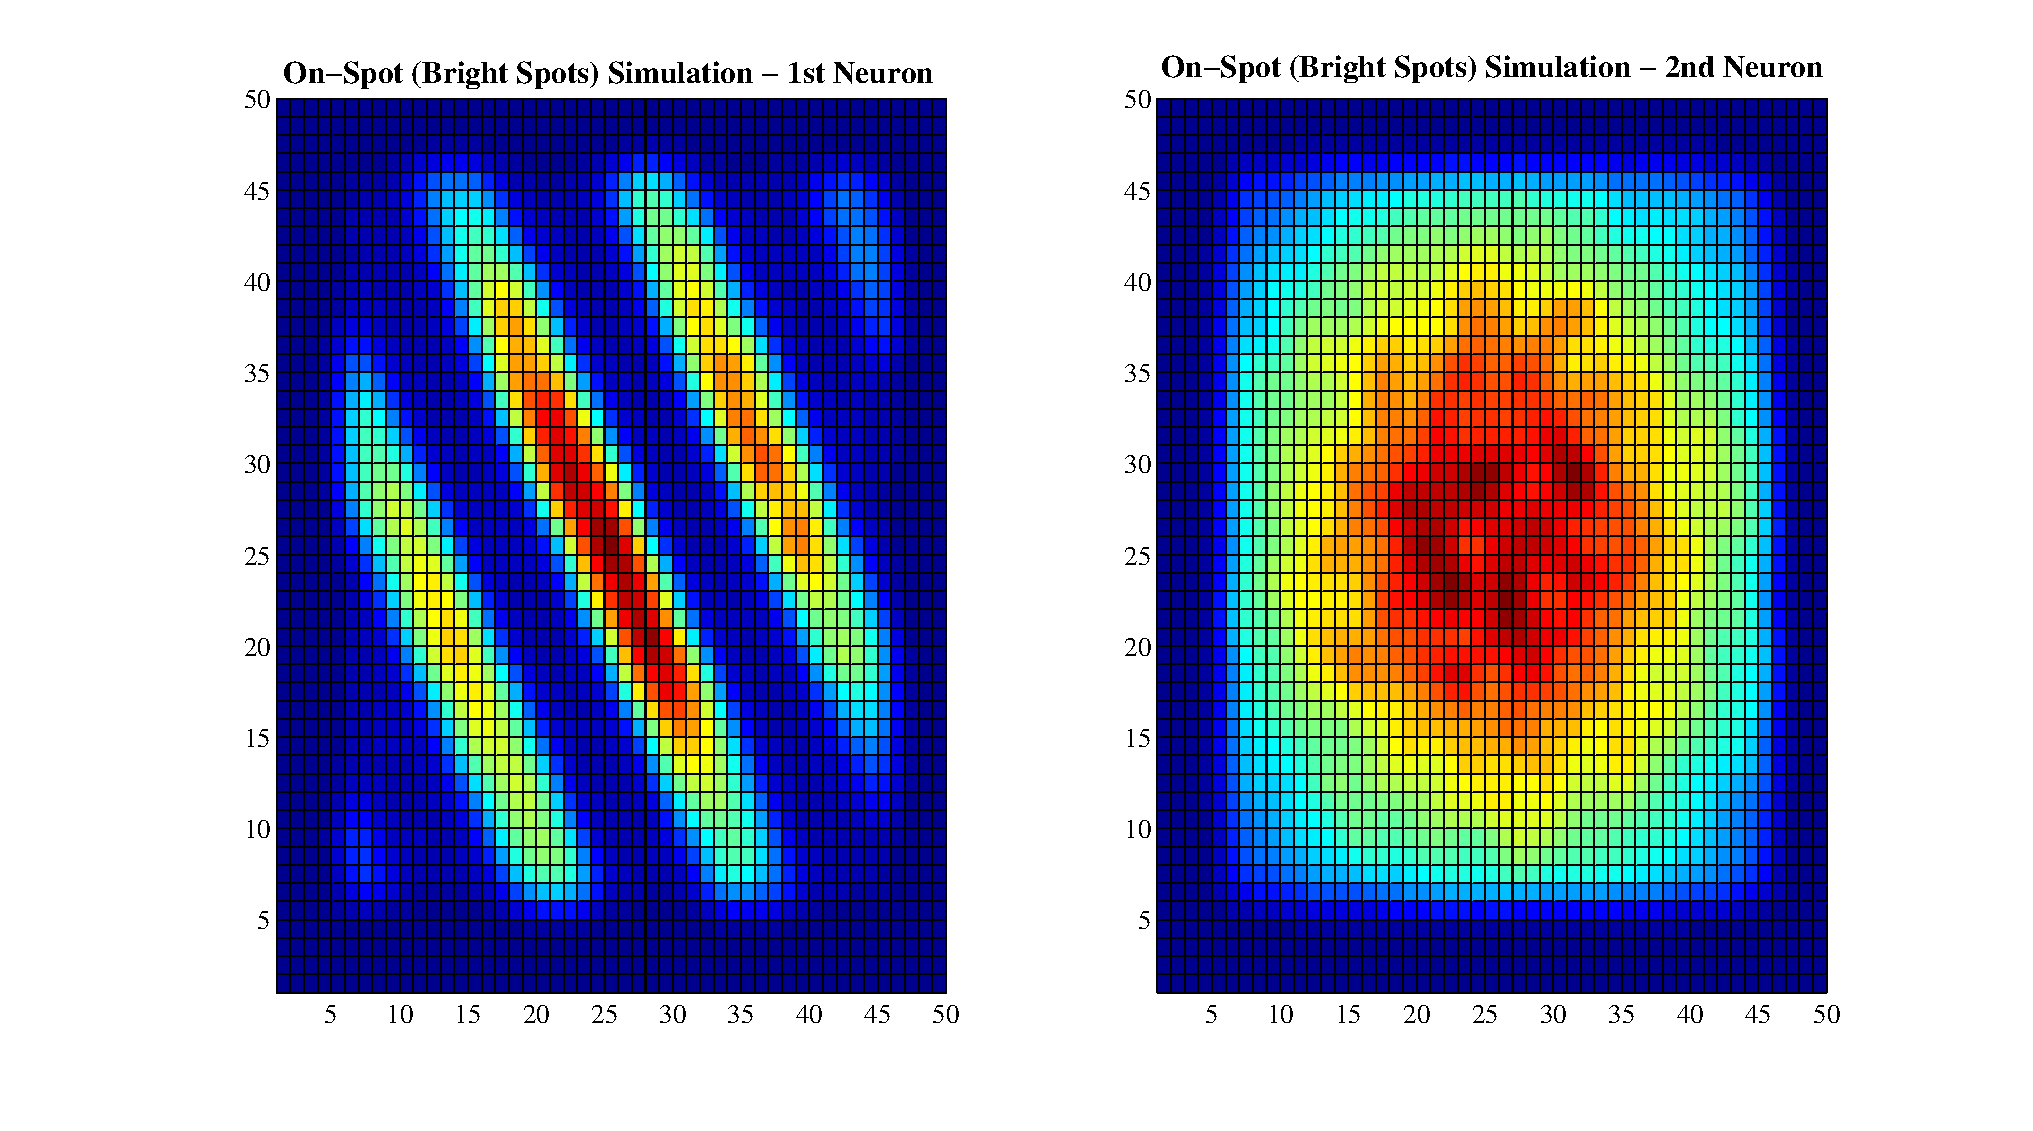
\includegraphics[width=\textwidth]{onspot.eps}
 % q7.eps: 0x0 pixel, 300dpi, 0.00x0.00 cm, bb=  -86   231   682   610
\begin{footnotesize}Graph 5, Weighted average responses of two neurons driven by bright spots, N=500. \end{footnotesize}
\end{center}

\setcounter{tocdepth}{1}
\textbf{4.Stimulating repeatedly with dark spots:} The stimuli function is $S=OffSpot(n)$. Same procudure as in step 3 is repeated, graph 6 is eliminated.

\begin{center}
 \includegraphics[width=\textwidth]{offspot.eps}
 % q7.eps: 0x0 pixel, 300dpi, 0.00x0.00 cm, bb=  -86   231   682   610
\begin{footnotesize}Graph 6, Weighted average responses of two neurons driven by dark spots, N=50000. \end{footnotesize}
\end{center}

\setcounter{tocdepth}{1}
\textbf{5.Stimulating repeatedly with noise:} The stimuli function is $S=WhiteNoise(n)$. Same procudure as in step 3 is repeated, graph 7 is eliminated.

\begin{center}
 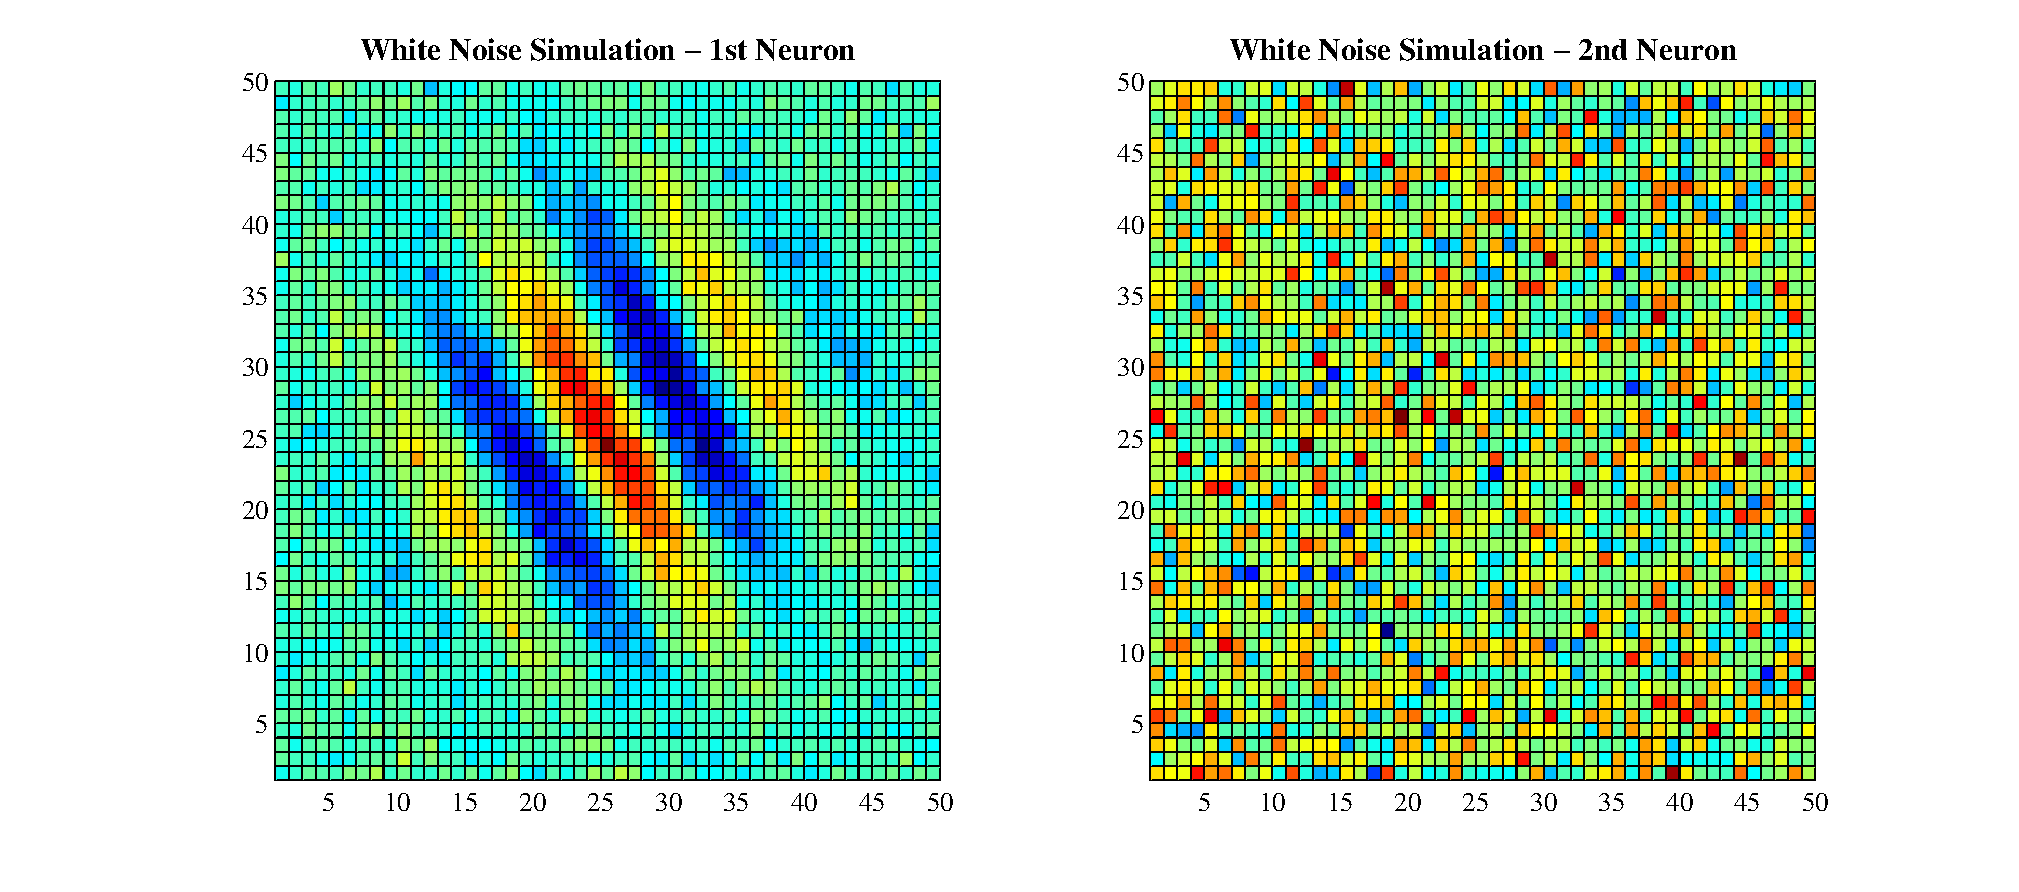
\includegraphics[width=\textwidth]{whitenoise.eps}
 % q7.eps: 0x0 pixel, 300dpi, 0.00x0.00 cm, bb=  -86   231   682   610
\begin{footnotesize}Graph 7, Weighted average responses of two neurons driven by dark white noise, N=50000. \end{footnotesize}
\end{center}

\section*{Discussion}

Graph 1 and 2 indicates that, the reponse of a neuron depends on the position of stimulus which triggers it. While the 1st neruon is well excited between 0 and 0.3$\pi$ radyan degrees at highest, the second one is at 0.2$\pi$ and 0.5$\pi$ radyan degrees. The frequency of stimulus is a bit higher at 2nd neuron in comparison to 2. Additinally the standart deviation $\sigma$ of 2nd neuron is relatively smaller than that of 1st neuron. Comparison of Graph 1 and 3 shows that, 1st neuron responses higher when it is triggered by bright bars rather than dark bars. However there is not a clear difference between 2nd neuron's responses to the dark and bright spots.

Graph 5,6 and 7 are plotted by obtaining a response weighted  average of the stimulus for two neurons, the type of stimuli differs on each graph. The average stimulations are all repsresented actually as 50 x 50 matrices, we have 2500 small square boxes on plots. Each box represent an average response, same colors represent same amount of response. For example; whereas blue color represents no response, orange color stands for the maximum response at Graph 5.\\

The first triggered neuron on Graph 5 has its maximum responses on some stripe shapes. The second neuron has its highest valued responses on same circles. The response of second neuron increases with decreasing radius of circles. Same analogy holds for graph 6 too. Here is the difference between Graph 5 and Graph 6: The 1st neruon gives more often responses to the dark spots (\textit{OffSpot}) compared to that of bright spots (\textit{OnSpot}). Number of stripes is higher at graph 6 and their colors are more distinctive. However, second neueron's response is higher to bright spots compared to dark spots. This can be understood from the fact that, the inner circular area of the highest response at Graph 5 is greater than that of Graph 6.\\

The last graph has a totally new type of stimuli called white noise. Graph 7 shows the response of 1st neruon, again in strike shapes. But this time strikes happen the most often, distance between them (analogous to standart deviation $\sigma$) is the least. On the other hand, there is no bare response shape for the second neruon. The first neuron could be more sensitive or higher developed to create distinctive response than the second one, or white noise stimulus is just not likely for the 2nd neuron.\\

The 1st neuron has some particular orientation and direction in its grating response. It could be either simple or complex cell. Since the response of 1st neuron to the on and off spots do not really differ (the strength of it might differ but orientation, shape etc. seem mainly very similar), the type is more analogous to the \textit{complex cell}. The 2nd neuron could be \textit{retinal ganglion cells}, it has small localized receptive fields and excited at the most in the inner circular part. \\

The advantage of different stimuli types is to help us to guess approximately the type of our mysterious neurons. The disadvantage is that, there does not exist a real stimuli response, we get an average for many trials. It is a bit far from reality, because in order to get reasonably explained plots, I had to get an average responce for each tiny square 50000 times! 



\end{document}
